\documentclass[9pt]{beamer}
\usepackage[utf8]{inputenc}
\usepackage[russian,english]{babel}
\usepackage{graphicx, epsfig}
\usepackage{amsmath,mathrsfs,amsfonts,amssymb}
\usepackage{subfig}
\usepackage{floatflt}
\usepackage{epic,ecltree}
\usepackage{mathtext}
\usepackage{fancybox}
\usepackage{fancyhdr}
\usepackage{multirow}
\usepackage{enumerate}
\usepackage{epstopdf}
\usepackage{multicol}
\usepackage{algorithm}
\usepackage[noend]{algorithmic}
\def\algorithmicrequire{\textbf{Input:}}
\def\algorithmicensure{\textbf{Output:}}
\usetheme{Singapore}%{Singapore}%{Warsaw}%{Warsaw}%{Darmstadt}
\usecolortheme{default}
\setbeamertemplate{footline}[page number]{}
\newcommand{\bx}{\mathbf{x}}
\newcommand{\by}{\mathbf{y}}
\newcommand{\bz}{\mathbf{z}}
\newcommand{\bw}{\mathbf{w}}
\newcommand{\ba}{\mathbf{a}}
\newcommand{\bb}{\mathbf{b}}
\newcommand{\bY}{\mathbf{Y}}
\newcommand{\bX}{\mathbf{X}}
\newcommand{\bu}{\mathbf{u}}
\newcommand{\bt}{\mathbf{t}}
\newcommand{\bp}{\mathbf{p}}
\newcommand{\bq}{\mathbf{q}}
\newcommand{\bc}{\mathbf{c}}
\newcommand{\bP}{\mathbf{P}}
\newcommand{\bT}{\mathbf{T}}
\newcommand{\bB}{\mathbf{B}}
\newcommand{\bQ}{\mathbf{Q}}
\newcommand{\bC}{\mathbf{C}}
\newcommand{\bE}{\mathbf{E}}
\newcommand{\bF}{\mathbf{F}}
\newcommand{\bU}{\mathbf{U}}
\newcommand{\bW}{\mathbf{W}}
\newcommand{\bbR}{\mathbb{R}}
\newcommand{\cA}{\mathcal{A}}
\newcommand{\bchi}{\boldsymbol{\chi}}
\newcommand{\bnu}{\boldsymbol{\nu}}
\newcommand{\bmu}{\boldsymbol{\mu}}
\newcommand{\bOne}{\boldsymbol{1}}
\newcommand{\bZero}{\boldsymbol{0}}
\newcommand{\btheta}{\boldsymbol{\theta}}
\newcommand{\bTheta}{\boldsymbol{\Theta}}
\newcommand{\argmin}{\mathop{\arg \min}\limits}
\newcommand{\argmax}{\mathop{\arg \max}\limits}
\newcommand{\T}{\mathsf{T}}

\newcommand\undermat[2]{%
	\makebox[0pt][l]{$\smash{\underbrace{\phantom{%
					\begin{matrix}#2\end{matrix}}}_{\text{$#1$}}}$}#2}

\newtheorem{statement}{Statement}

\titlegraphic{
\includegraphics[width=2cm]{figs/mipt_logo}~%
	
\includegraphics[width=2cm]{figs/sk_logo}
}

% отображать название слайда слева
\setbeamertemplate{frametitle}[default][left]

\usepackage{tikz-cd}
%\definecolor{beamer@blendedblue}{RGB}{15,120,80}
%----------------------------------------------------------------------------------------------------------
\title[\hbox to 56mm{  \hfill\insertframenumber\,/\,\inserttotalframenumber}]
{\\ \vspace{1.5cm} Feature Selection for Miltivariate Correlated ECoG-based data}
\author[Roman Isachenko]{\\ 
	\vspace{.4cm}
	Roman Isachenko}
\institute[SkolTech]{Skoltech advisor: Maxim Fedorov \\ 
	\vspace{0.1cm}
	 MIPT advisor: Vadim Strijov
}
\date{May 16, 2018.}
%--------------------------------------------------------------------------------
\begin{document}
%--------------------------------------------------------------------------------
\begin{frame}
%\thispagestyle{empty}
\titlepage
\end{frame}
%--------------------------------------------------------------------------------
\begin{frame}{Signal decoding problem}
	\begin{block}{Goal}
		\begin{itemize}
			\item Investigate dependencies in input and target spaces for signal decoding problem.
			\item Build a stable model for time series decoding in the case of multicorrelated object description.
		\end{itemize}
	\end{block}
	\begin{block}{Challenge}
		\begin{itemize}
			\item Measurements of spatial-temporal data are interacted since sensors are close to each other.
			\item Target variable is a vector whose elements are dependent.
		\end{itemize}
	\end{block}
	\begin{block}{Solution}
		Propose feature selection algorithms which take into account dependencies in both input and target spaces. 
	\end{block}
\end{frame}
%--------------------------------------------------------------------------------
\begin{frame}{Related works}
	\begin{itemize}
		\item Katrutsa A., Strijov V. Comprehensive study of feature selection methods to solve multicollinearity problem according to evaluation criteria // \textit{Expert Systems with Applications} 76, 2017.
		\vfill
		\item Li J. et al. Feature selection: A data perspective //\textit{ACM Computing Surveys (CSUR)} 50(6), 2017.
		\vfill
		\item Eliseyev A. et al. Iterative N-way partial least squares for a binary self-paced brain–computer interface in freely moving animals //\textit{Journal of neural engineering} 4(8), 2011.
		\vfill
		\item Rodriguez-Lujan I. et al. Quadratic programming feature selection // \textit{Journal of Machine Learning Research} 11(Apr), 2010.
		\vfill
		\item Motrenko A., Strijov V. Multi-way Feature Selection for ECoG-based Brain-Computer Interface // \textit{Expert Systems with Applications} Submitted to the journal.
	\end{itemize}
\end{frame}
%--------------------------------------------------------------------------------
\begin{frame}{Application: Brain Computer Interface (BCI)}
	\begin{minipage}{0.58\linewidth}
		\begin{block}{Aim}
		Develop systems to help people with a severe motor control disability recover mobility.
		\end{block}
	\begin{block}{Hypothesis}
	"When we imagine making a movement, we trigger the same electrical activity in the motor cortex of the brain as when we actually perform that activity."$^*$
	\end{block}
	\begin{block}{Solution}
	Record electrical signals~-- electrocorticograms (ECoG), decode them to drive complex objects, for example, to move the limbs of an exoskeleton. 
	\end{block}
	$^*$ \url{http://clinatec.fr}
	\end{minipage}%
\begin{minipage}{0.4\linewidth}
	\centering
	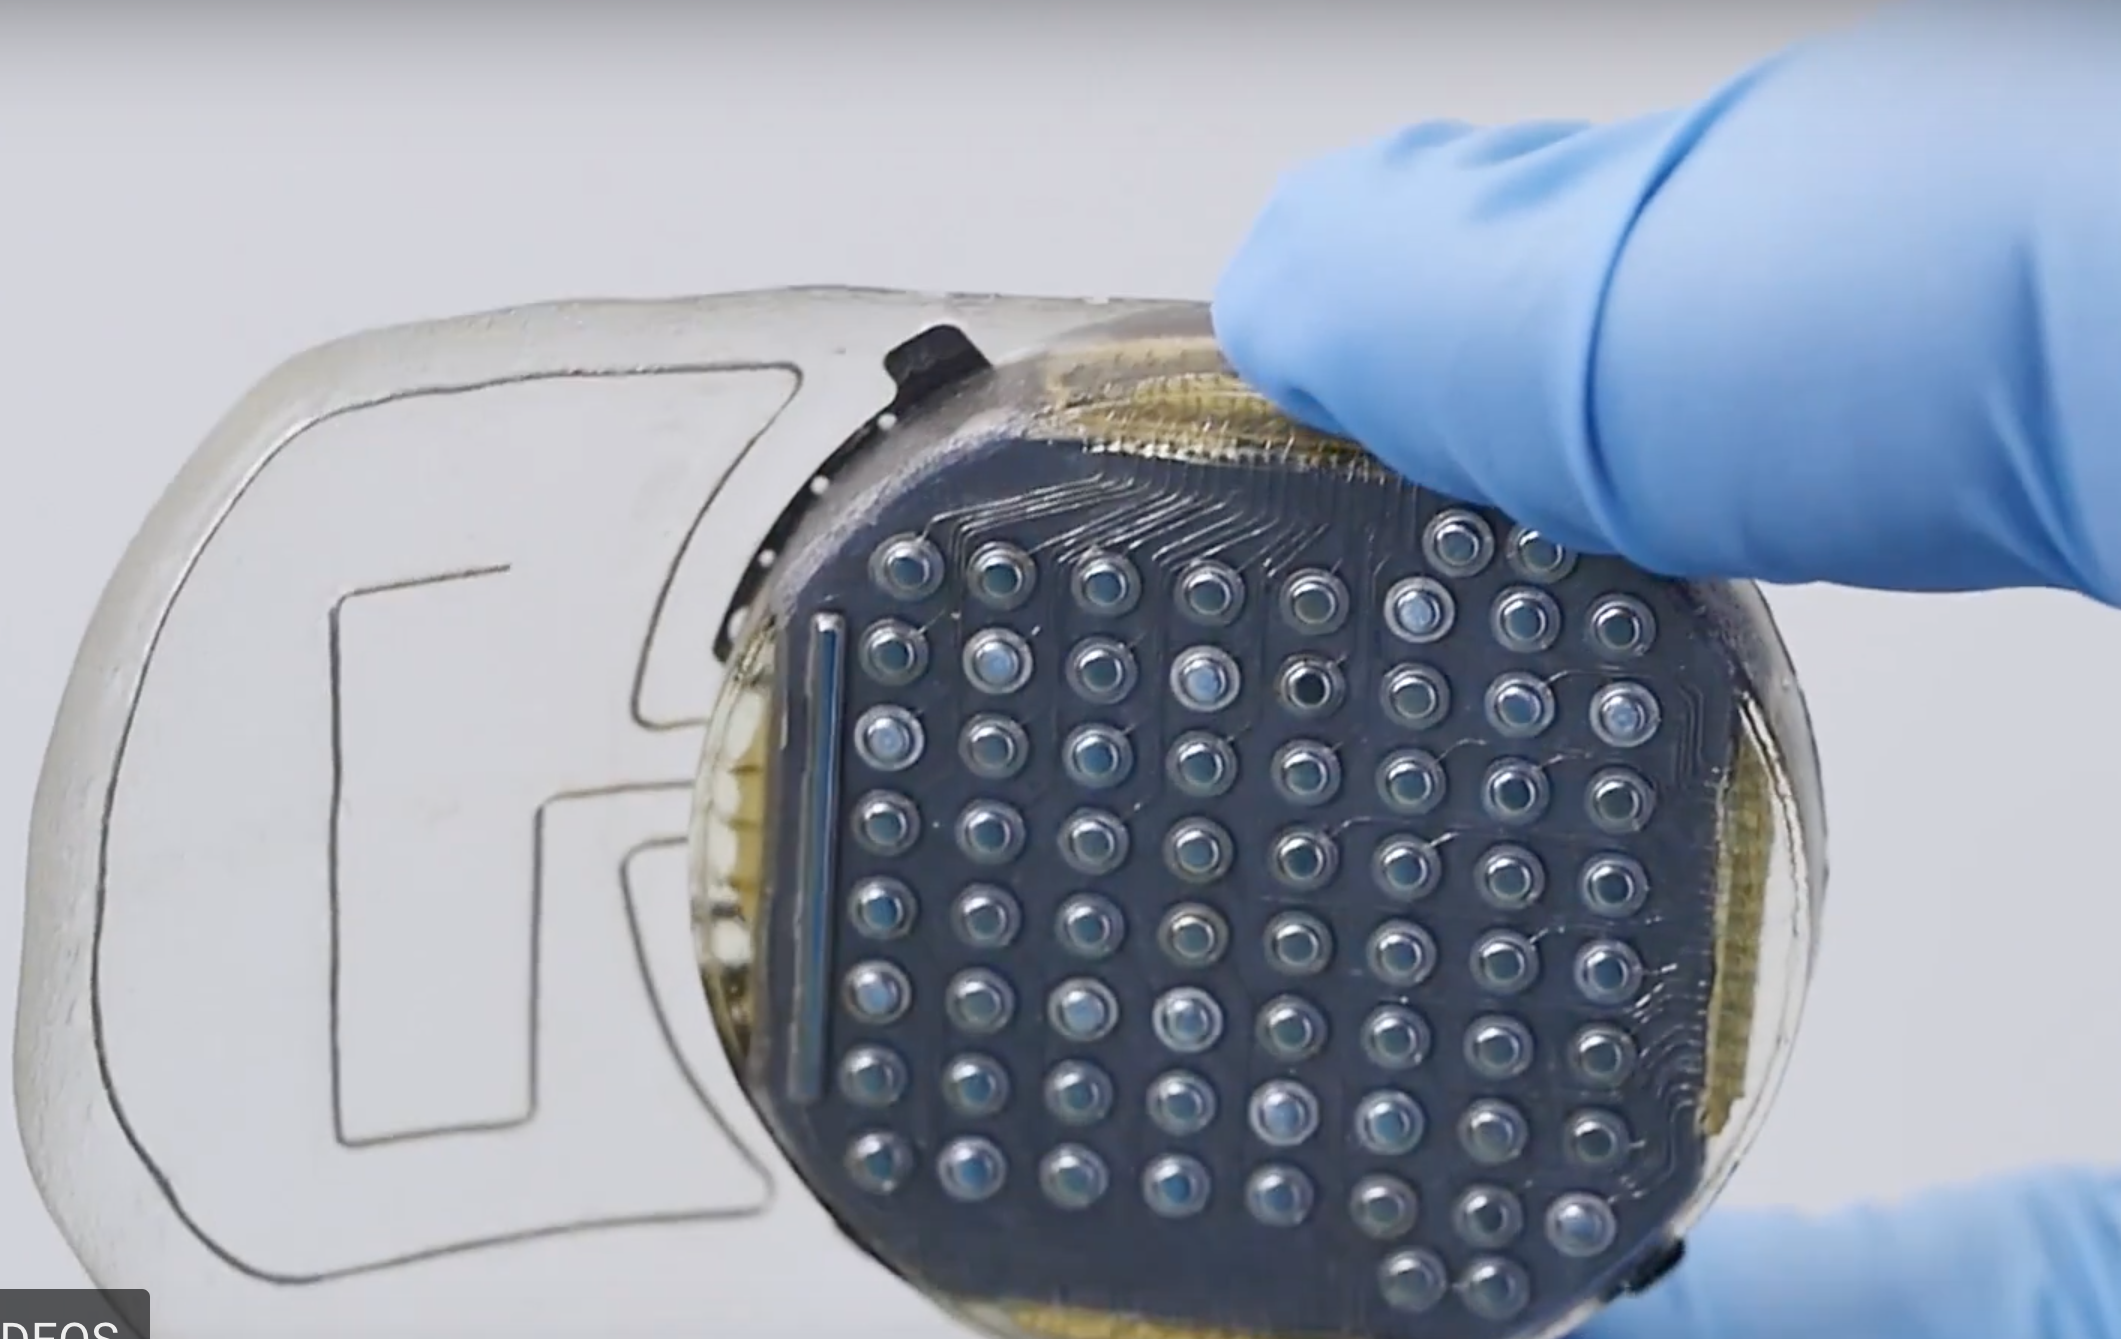
\includegraphics[width=0.9\linewidth]{figs/deviceClinatec} \\
	\vspace{0.5cm}
	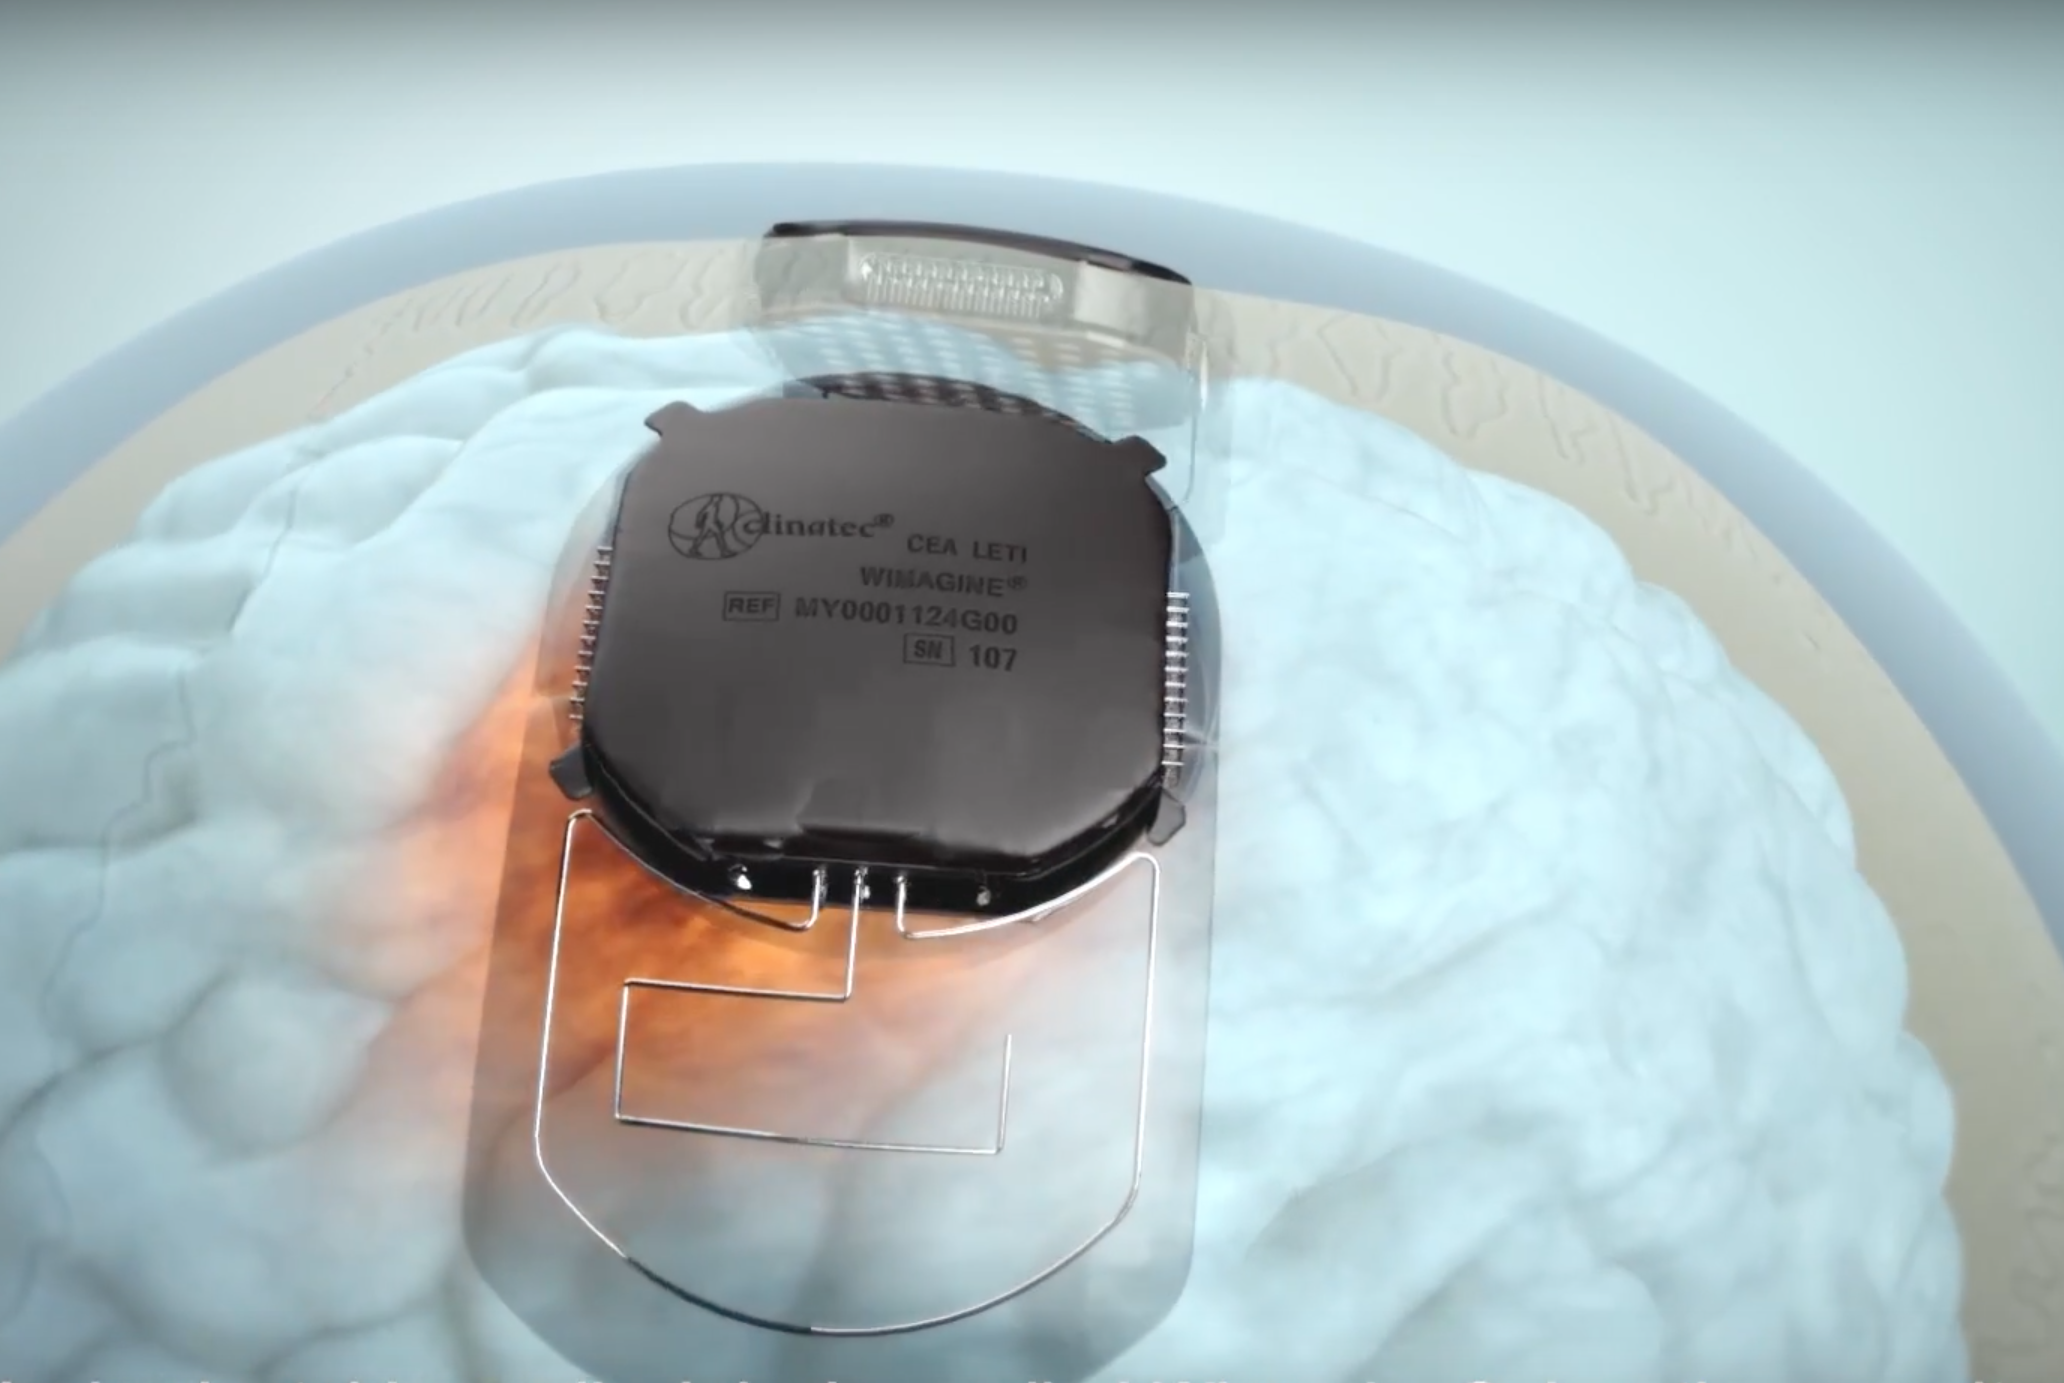
\includegraphics[width=0.9\linewidth]{figs/brainClinatec}
\end{minipage}
\vspace{0.3cm} \\
\hrulefill \\
\small{Eliseyev A. et al. CLINATEC BCI platform based on the ECoG-recording implant WIMAGINE and the innovative signal-processing: preclinical results, 2014.}
\end{frame}
%--------------------------------------------------------------------------------
\begin{frame}{Multivariate regression}
	\begin{block}{Given}
	Dataset $\left( \bX, \bY \right)$, design matrix~$\bX \in \bbR^{m \times n}$, target matrix~$\bY \in \bbR^{m \times r}$,
	\[
	\bX = [\bchi_1, \dots, \bchi_n]; \quad \bY =  [\bnu_1, \dots, \bnu_r].
	\]
	\vspace{-0.7cm}
	\end{block}

\begin{block}{Model}
	Forecast a dependent variable $\by \in \bbR^r$ from an independent input object $\bx \in \bbR^n$
	\[
	\by = \bTheta \bx+ \boldsymbol{\varepsilon}, \quad \bTheta \in \bbR^{r \times n}.
	\]
	\vspace{-0.7cm}
\end{block}
	\begin{block}{Loss function}
	\[
	\mathcal{L}(\bTheta | \bX, \bY) = {\left\| \underset{m \times r}{\mathbf{Y}}  - \underset{m \times n}{\bX} \cdot \underset{r \times n}{\bTheta}^{\T} \right\| }_2^2 \rightarrow\min_{\bTheta}.
	\label{eq:error_function}
	\]
	\[
	\bTheta^{\T} = (\bX^{\T} \bX)^{-1} \bX^{\T} \bY.
	\]
	\end{block}
	The linear dependent columns of the matrix $\bX$ leads to an instable solution. \\
	To avoid the strong linear dependence, feature selection techniques are used.
\end{frame}

%--------------------------------------------------------------------------------
\begin{frame}{Feature selection problem}
\begin{block}{Goal}
Find a boolean vector~$\ba = \{0, 1\}^n$ of indicators for selected features. 
\end{block}
\begin{block}{Feature selection error function}
	\vspace{-0.2cm}
\[
\ba = \argmin_{\ba' \in \{0, 1\}^n} S(\ba' | \bX, \bY).
\]
\vspace{-0.5cm}
\end{block}
\begin{block}{Relaxed problem}
	From discrete domain $\{0, 1\}^n$ to continuous relaxation $[0, 1]^n$:
	\[
	\bz = \argmin_{\bz' \in [0, 1]^n} S(\bz' | \bX, \bY), \quad 
	a_j = [z_j > \tau].
\]
\end{block}
Once the solution~$\ba$ is known:
\[
\mathcal{L}(\bTheta_{\ba} | \bX_{\ba}, \bY) = {\left\| \mathbf{Y} - \bX_{\ba}\bTheta^{\T}_{\ba} \right\| }_2^2 \rightarrow\min_{\bTheta_{\ba}},
\]
where the subscript~$\ba$ indicates the submatrix with the columns for which~$a_j = 1$.
\end{frame}
%--------------------------------------------------------------------------------
\begin{frame}{Quadratic Programming Feature Selection}
	\[
	\| \bnu - \bX \btheta\|_2^2 \rightarrow\min_{\btheta \in \bbR^{n}}.
	\]
	\vspace{-0.3cm}
	\begin{block}{Quadratic programming problem}
	\vspace{-0.3cm}
	\[
	S(\bz' | \bX, \bnu)	= (1 - \alpha) \cdot \underbrace{\bz^{\T} \bQ \bz}_{\text{Sim}(\bX)} - \alpha \cdot \underbrace{\vphantom{()} \mathbf{b}^{\T} \bz}_{\text{Rel}(\bX, \bnu)} \rightarrow \min_{\substack{\bz \geq \bZero_n \\ \bOne_n^{\T} \bz=1}}.
	\]
	\end{block}
		\begin{itemize}
			\item $\bz \in [0, 1]^n$ -- feature importances;
			\item $\bQ \in \bbR^{n \times n}$ -- pairwise feature similarities;
			\item $\mathbf{b} \in \bbR^n$ -- feature relevances to the target vector.
		\end{itemize}
		\[
		\bQ = \left[\left|\text{corr}(\bchi_i, \bchi_j)\right|\right]_{i,j=1}^n, \quad
		\bb = \left[\left|\text{corr}(\bchi_i, \bnu)\right|\right]_{i=1}^n.
		\]
\vspace{-0.2cm}
\begin{block}{Statement}
	In the case of semidefinite matrix $\bQ$ the QPFS problem is convex. Shift spectrum for semidefinite relaxation:
\end{block}
\begin{equation*}
\bQ \rightarrow \bQ - \lambda_{\min} \mathbf{I}.
\end{equation*}
\end{frame}
%--------------------------------------------------------------------------------
\begin{frame}{Multivariate QPFS}
	\begin{block}{Feature selection error function}
	\[
	\bz = \argmin_{\bz' \in [0, 1]^n} S(\bz' | \bX, \bY) = \argmin_{\bz \geq \bZero_n, \, \bOne_n^{\T}\bz=1} \bigl[(1 - \alpha) \cdot \bz^{\T} \bQ \bz - \alpha \cdot \mathbf{b}^{\T} \bz \bigr].
	\]
\end{block}
\begin{block}{Relevance Aggregation (RelAgg)}
\[
\bb = \left[\left|\text{corr}(\bchi_i, \bnu)\right|\right]_{i=1}^n \rightarrow \bb = \left[\sum_{k=1}^r\left|\text{corr}(\bchi_i, \bnu_k)\right|\right]_{i=1}^n.
\]
\end{block}

This approach does not use the dependencies in the columns of the matrix $\bY$. 
\end{frame}
%--------------------------------------------------------------------------------
\begin{frame}{Symmetric Importance (SymImp)}
Penalize correlated targets by $\text{Sim} (\bY)$
\[
\alpha_1 \cdot \underbrace{\bz_x^{\T} \bQ_x \bz_x}_{\text{Sim}(\bX)} - \alpha_2 \cdot \underbrace{\bz_x^{\T} \bB \bz_y}_{\text{Rel}(\bX, \bY)} + \alpha_3 \cdot \underbrace{\bz_y^{\T} \bQ_y \bz_y}_{\text{Sim}(\bY)} \rightarrow \min_{\substack{\bz_x \geq \bZero_n, \, \bOne_n^{\T}\bz_x=1 \\ \bz_y \geq \bZero_r, \, \bOne_r^{\T}\bz_y=1}}.
\]
\[
\bQ_x = \left[ \left| \text{corr}(\bchi_i, \bchi_j) \right| \right]_{i,j=1}^n, \,
\bQ_y = \left[ \left| \text{corr}(\bnu_i, \bnu_j) \right| \right]_{i,j=1}^r, \,
\bB =  \left[ \left| \text{corr}(\bchi_i, \bnu_j) \right| \right]_{\substack{i=1, \dots, n \\ j=1, \dots, r}}.
\]
\[
\alpha_1 + \alpha_2 + \alpha_3 = 1 \quad \alpha_i \geq 0, \, i = 1, 2, 3.
\] 

\begin{statement}
	Balance between $\text{Sim}(\bX)$, $\text{Rel}(\bX, \bY)$, and $\text{Sim}(\bY)$ is achieved by:
	\vspace{-0.2cm}
	\[
		\alpha_1 \propto \overline{\bQ}_y \overline{\bB}; \quad
		\alpha_2 \propto \overline{\bQ}_x \overline{\bQ}_y; \quad
		\alpha_3  \propto \overline{\bQ}_x \overline{\bB},
	\]
	where $\overline{\bQ}_x$, $\overline{\bB}$, $\overline{\bQ}_y$ are mean values of~$\bQ_x$, $\bB$, and $\bQ_y$, respectively.
\end{statement}
\end{frame}
%--------------------------------------------------------------------------------
\begin{frame}{MinMax / MaxMin}
	SymImp penalizes targets that are correlated and are not sufficiently explained by the features. 
	\[
	\alpha_1 \cdot \underbrace{\bz_x^{\T} \bQ_x \bz_x}_{\text{Sim}(\bX)} - \alpha_2 \cdot \underbrace{\vphantom{()} \bz_x^{\T}\mathbf{B} \bz_y}_{\text{Rel}(\bX, \bY)} \rightarrow \min_{\substack{\bz_x \geq \bZero_n, \\ \bOne_n^{\T}\bz_x=1}}; \quad
	\alpha_3 \cdot \underbrace{\bz_y^{\T} \bQ_y \bz_y}_{\text{Sim}(\bY)} + \alpha_2 \cdot \underbrace{\vphantom{()} \bz_x^{\T} \mathbf{B} \bz_y}_{\text{Rel}(\bX, \bY)} \rightarrow \min_{\substack{\bz_y \geq \bZero_r,  \\ \bOne_r^{\T}\bz_y=1}}.
	\]
	\vspace{-0.2cm}
	\begin{block}{Minimax problem}
	\vspace{-0.5cm}
	\[
	\min_{\substack{\bz_x \geq \bZero_n \\ \bOne_n^{\T}\bz_x=1}} 	\max_{\substack{\bz_y \geq \bZero_r \\ \bOne_r^{\T}\bz_y=1}} \left(\text {or} \, \max_{\substack{\bz_y \geq \bZero_r \\ \bOne_r^{\T}\bz_y=1}} \min_{\substack{\bz_x \geq \bZero_n \\ \bOne_n^{\T}\bz_x=1}}\right) \left[\alpha_1 \cdot \underbrace{\bz_x^{\T} \bQ_x \bz_x}_{\text{Sim}(\bX)} - \alpha_2 \cdot \underbrace{\bz_x^{\T} \bB \bz_y}_{\text{Rel}(\bX, \bY)} - \alpha_3 \cdot \underbrace{\bz_y^{\T} \bQ_y \bz_y}_{\text{Sim}(\bY)}\right].
	\]
	\end{block}
	\vspace{-0.4cm}
	\begin{theorem}
		For positive definite matrices $\bQ_x$ and $\bQ_y$ the max-min and min-max problems have the same optimal value. 
	\end{theorem}
	\vspace{-0.2cm}
	\begin{theorem}
		Minimax problem is equivalent to the quadratic problem with $n + r + 1$ variables.
	\end{theorem}
	Shift spectrum to obtain the convex problem.

\end{frame}
%--------------------------------------------------------------------------------
\begin{frame}{Maximum Relevance (MaxRel)}
	Drop the term~$\text{Sim}(\bY)$. 
	\begin{block}{Minimax problem}
	\[
		\min_{\substack{\bz_x \geq \bZero_n \\ \bOne_n^{\T}\bz_x=1}} 	\max_{\substack{\bz_y \geq \bZero_r \\ \bOne_r^{\T}\bz_y=1}} \left[ (1 - \alpha) \cdot \bz_x^{\T} \bQ_x \bz_x - \alpha \cdot \bz_x^{\T} \bB \bz_y \right].
	\]
	\end{block}
	\begin{theorem}
		For positive definite matrices $\bQ_x$ the max-min and min-max problems have the same optimal value and the final quadratic problem is convex. 
	\end{theorem}
\begin{statement}
	For the case $r=1$ the proposed strategies SymImp, MinMax, MaxMin, MaxRel coincide with the original QPFS algorithm.
\end{statement}
\end{frame}
%--------------------------------------------------------------------------------
\begin{frame}{Summary}
\begin{table}
	\centering
	\footnotesize{
		\begin{tabular}{l|c|c}
			\hline
			\textbf{Algorithm} & \textbf{Strategy} & \textbf{Error function $S(\bz | \bX, \bY)$} \\
			\hline && \\ [-.5em]
			RelAgg & $\min \bigl[ \text{Sim}(\bX) - \text{Rel}(\bX, \bY) \bigr] $ & $\min\limits_{\bz_x} \bigl[ (1 - \alpha) \cdot \bz_x^{\T} \bQ_x \bz_x - \alpha \cdot \bz_x^{\T} \bB \bOne_r \bigr] $ \\ 
			\hline&&\\[-.5em]
			SymImp & $\begin{aligned} \min \, \bigl[ \text{Sim}(\bX) & - \text{Rel}(\bX, \bY) \\ & + \text{Sim}(\bY) \bigr] \end{aligned}$ & $ \min\limits_{\bz_x, \, \bz_y} \left[ \alpha_1 \cdot \bz_x^{\T} \bQ_x \bz_x - \alpha_2 \cdot \bz_x^{\T} \bB \bz_y + \alpha_3 \cdot \bz_y^{\T} \bQ_y \bz_y \right] $\\ 
			\hline&&\\ [-.5em]
			MinMax & $\begin{aligned} &\min \, \bigl[ \text{Sim}(\bX) - \text{Rel}(\bX, \bY) \bigr]  \\ & \max \bigl[\text{Rel}(\bX, \bY) + \text{Sim}(\bY) \bigr] \end{aligned}$ & $	\min\limits_{\bz_x} 	\max\limits_{\bz_y} \bigl[\alpha_1 \cdot \bz_x^{\T} \bQ_x \bz_x - \alpha_2 \cdot \bz_x^{\T} \bB \bz_y - \alpha_3 \cdot \bz_y^{\T} \bQ_y \bz_y \bigr]$ \\ 
			\hline&&\\ 
			MaxMin & $\begin{aligned} &\max \bigl[\text{Rel}(\bX, \bY) + \text{Sim}(\bY) \bigr] \\ & \min \, \bigl[ \text{Sim}(\bX) - \text{Rel}(\bX, \bY) \bigr]  \end{aligned}$ & $\max\limits_{\bz_y} \min\limits_{\bz_x} \bigl[\alpha_1 \cdot \bz_x^{\T} \bQ_x \bz_x - \alpha_2 \cdot \bz_x^{\T} \bB \bz_y - \alpha_3 \cdot \bz_y^{\T} \bQ_y \bz_y \bigr]$\\ 
			\hline&&\\ [-.5em]
			MaxRel & $\begin{aligned} &\min \, \bigl[ \text{Sim}(\bX) - \text{Rel}(\bX, \bY) \bigr]  \\ & \max \bigl[\text{Rel}(\bX, \bY) \bigr] \end{aligned}$& $\min\limits_{\bz_x} 	\max\limits_{\bz_y} \bigl[ (1 - \alpha) \cdot \bz_x^{\T} \bQ_x \bz_x - \alpha \cdot \bz_x^{\T} \bB \bz_y \bigr]$ \\ 
			\hline
	\end{tabular}}
\end{table}
\end{frame}
%--------------------------------------------------------------------------------
\begin{frame}{Computational experiment}
\begin{figure}
	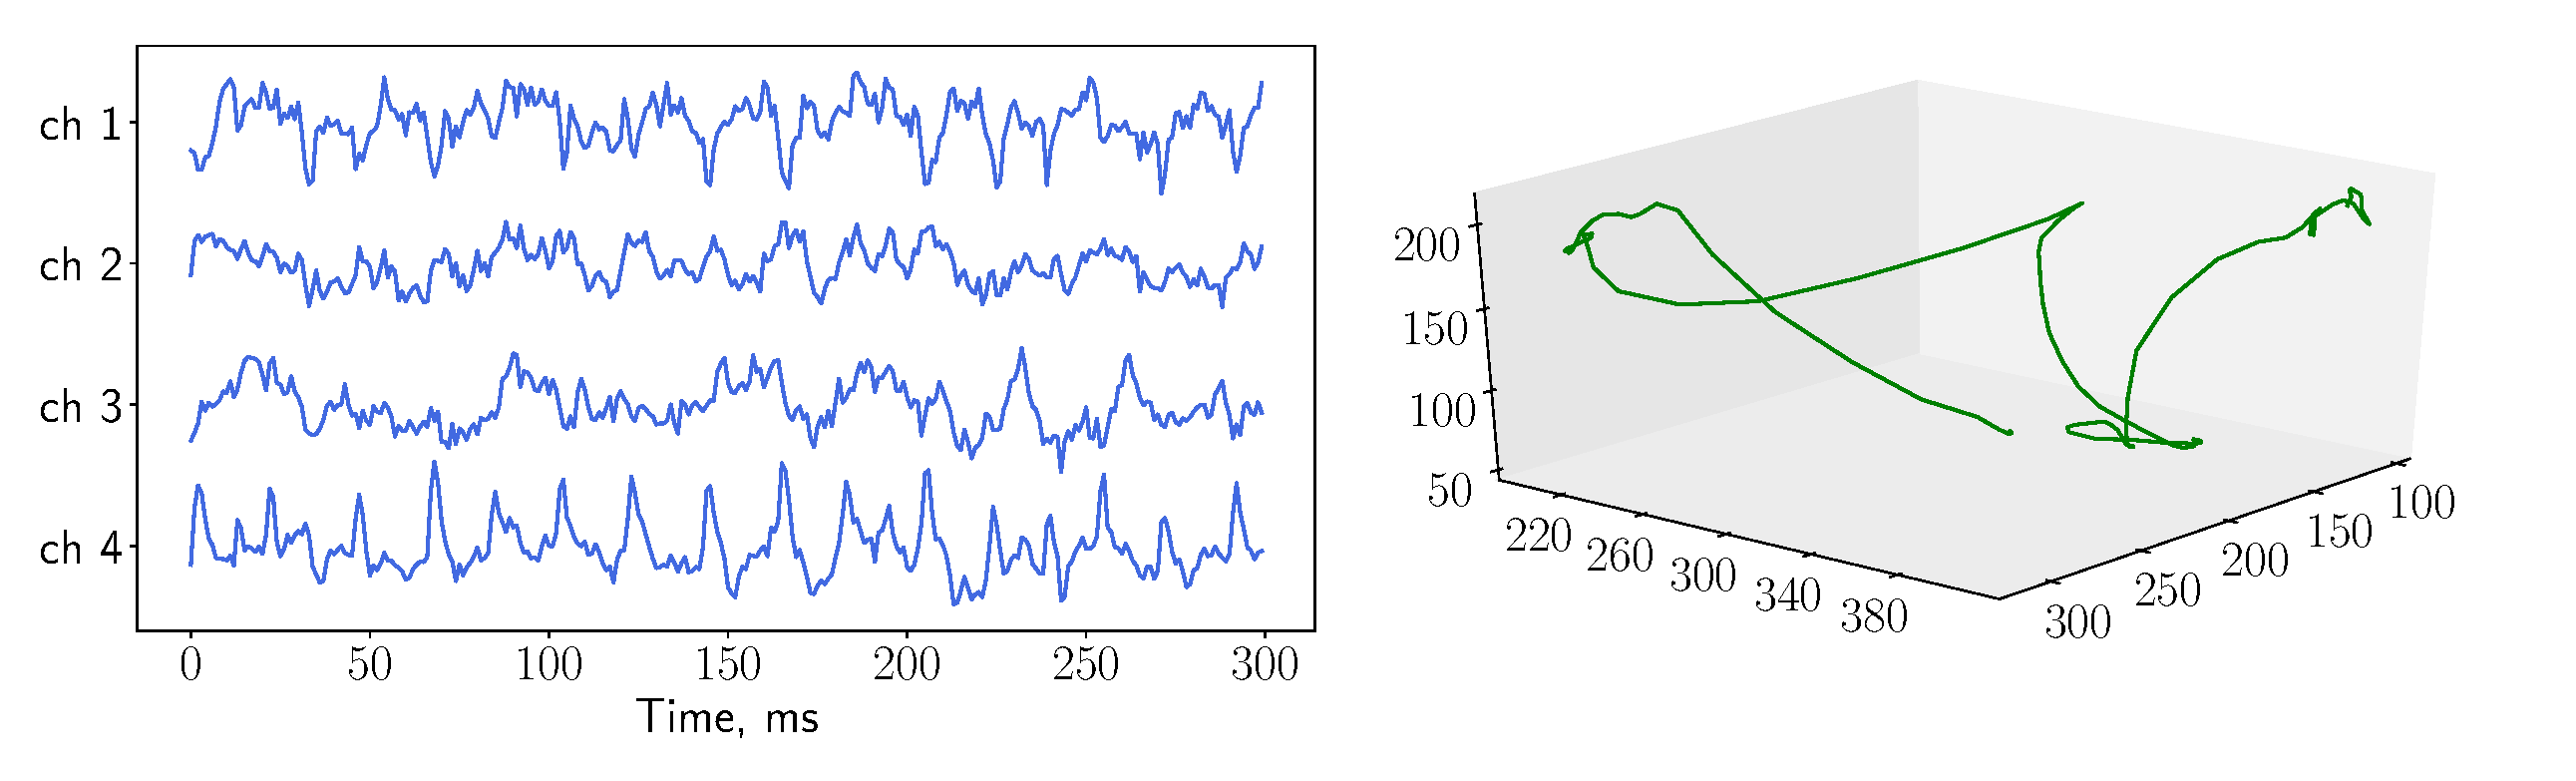
\includegraphics[width=\linewidth]{figs/ecog_data}
\end{figure}
\begin{minipage}{.55\linewidth}
\[
	\bX \in \bbR^{m \times (32 \cdot 27)}; \quad
	\bY \in \bbR^{m \times 3k}.
\]
\vspace{0.1cm}
\[
	\bY = 
	\begin{pmatrix}
	x_1 \,\, y_1 \,\, z_1 & \dots & x_{k\hphantom{+1}} \,\, y_{k\hphantom{+1}} \,\, z_{k\hphantom{+1}}\\
	x_2 \,\, y_2 \,\, z_2 & \dots & x_{k + 1} \,\, y_{k + 1} \,\, z_{k + 1}\\
	 \dots & \dots & \dots  \\
	x_m \, y_m \, z_m & \dots & x_{m + k} \, y_{m + k} \, z_{m + k}
	\end{pmatrix}
\]
\end{minipage}%
\begin{minipage}{.43\linewidth}
	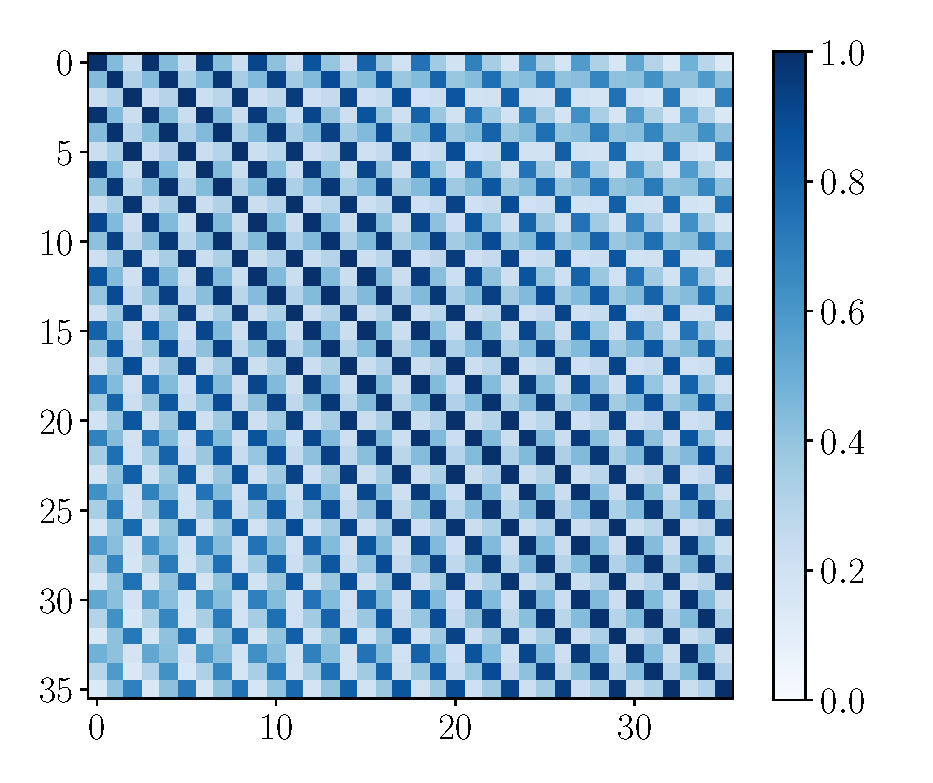
\includegraphics[width=\linewidth]{figs/Y_corr_matrix.eps}
	\begin{center}
		\vspace{-0.4cm}
		$\bY$ correlation matrix
		\vspace{-0.4cm}
	\end{center}
\end{minipage}
\vspace{0.5cm}

\hrulefill \\
\url{http://neurotycho.org}
\end{frame}
%--------------------------------------------------------------------------------
\begin{frame}{Metrics}

\begin{block}{RMSE}
	The prediction quality:
	\[
	\text{RMSE}(\bY, \widehat{\bY}_{\ba}) = \sqrt{\text{MSE} (\bY, \widehat{\bY}_{\ba})} =  \| \bY - \widehat{\bY}_{\ba} \|_2, \quad \text{where} \quad \widehat{\bY}_{\ba} = \bX_{\ba} \bTheta_{\ba}^{\T}.
	\]
\end{block}

\begin{block}{Multicorrelation}
Mean value of miltiple correlation coefficient:
\[
R^2 = \frac{1}{r} \text{tr} \left( \bC^{\T} \mathbf{R}^{-1} \bC \right); \quad \bC = [ \text{corr}(\bchi_i, \bnu_j)]_{\substack{i=1, \dots, n \\ j=1, \dots, r}}, \, \mathbf{R} = [ \text{corr}(\bchi_i, \bchi_j)]_{i, j = 1}^n.
\]
\end{block}
\begin{block}{BIC}
Bayesian Information Criteria is a trade-off between prediction quality and the number of selected features $\|\ba\|_0$:
\[
\text{BIC} = m \ln \left( \text{MSE} ( \bY, \widehat{\bY}_{\cA})\right) + \| \ba \|_0 \cdot \log m.
\]
\end{block}
\end{frame}
%--------------------------------------------------------------------------------
\begin{frame}{Metrics evaluation}
	\begin{figure}
		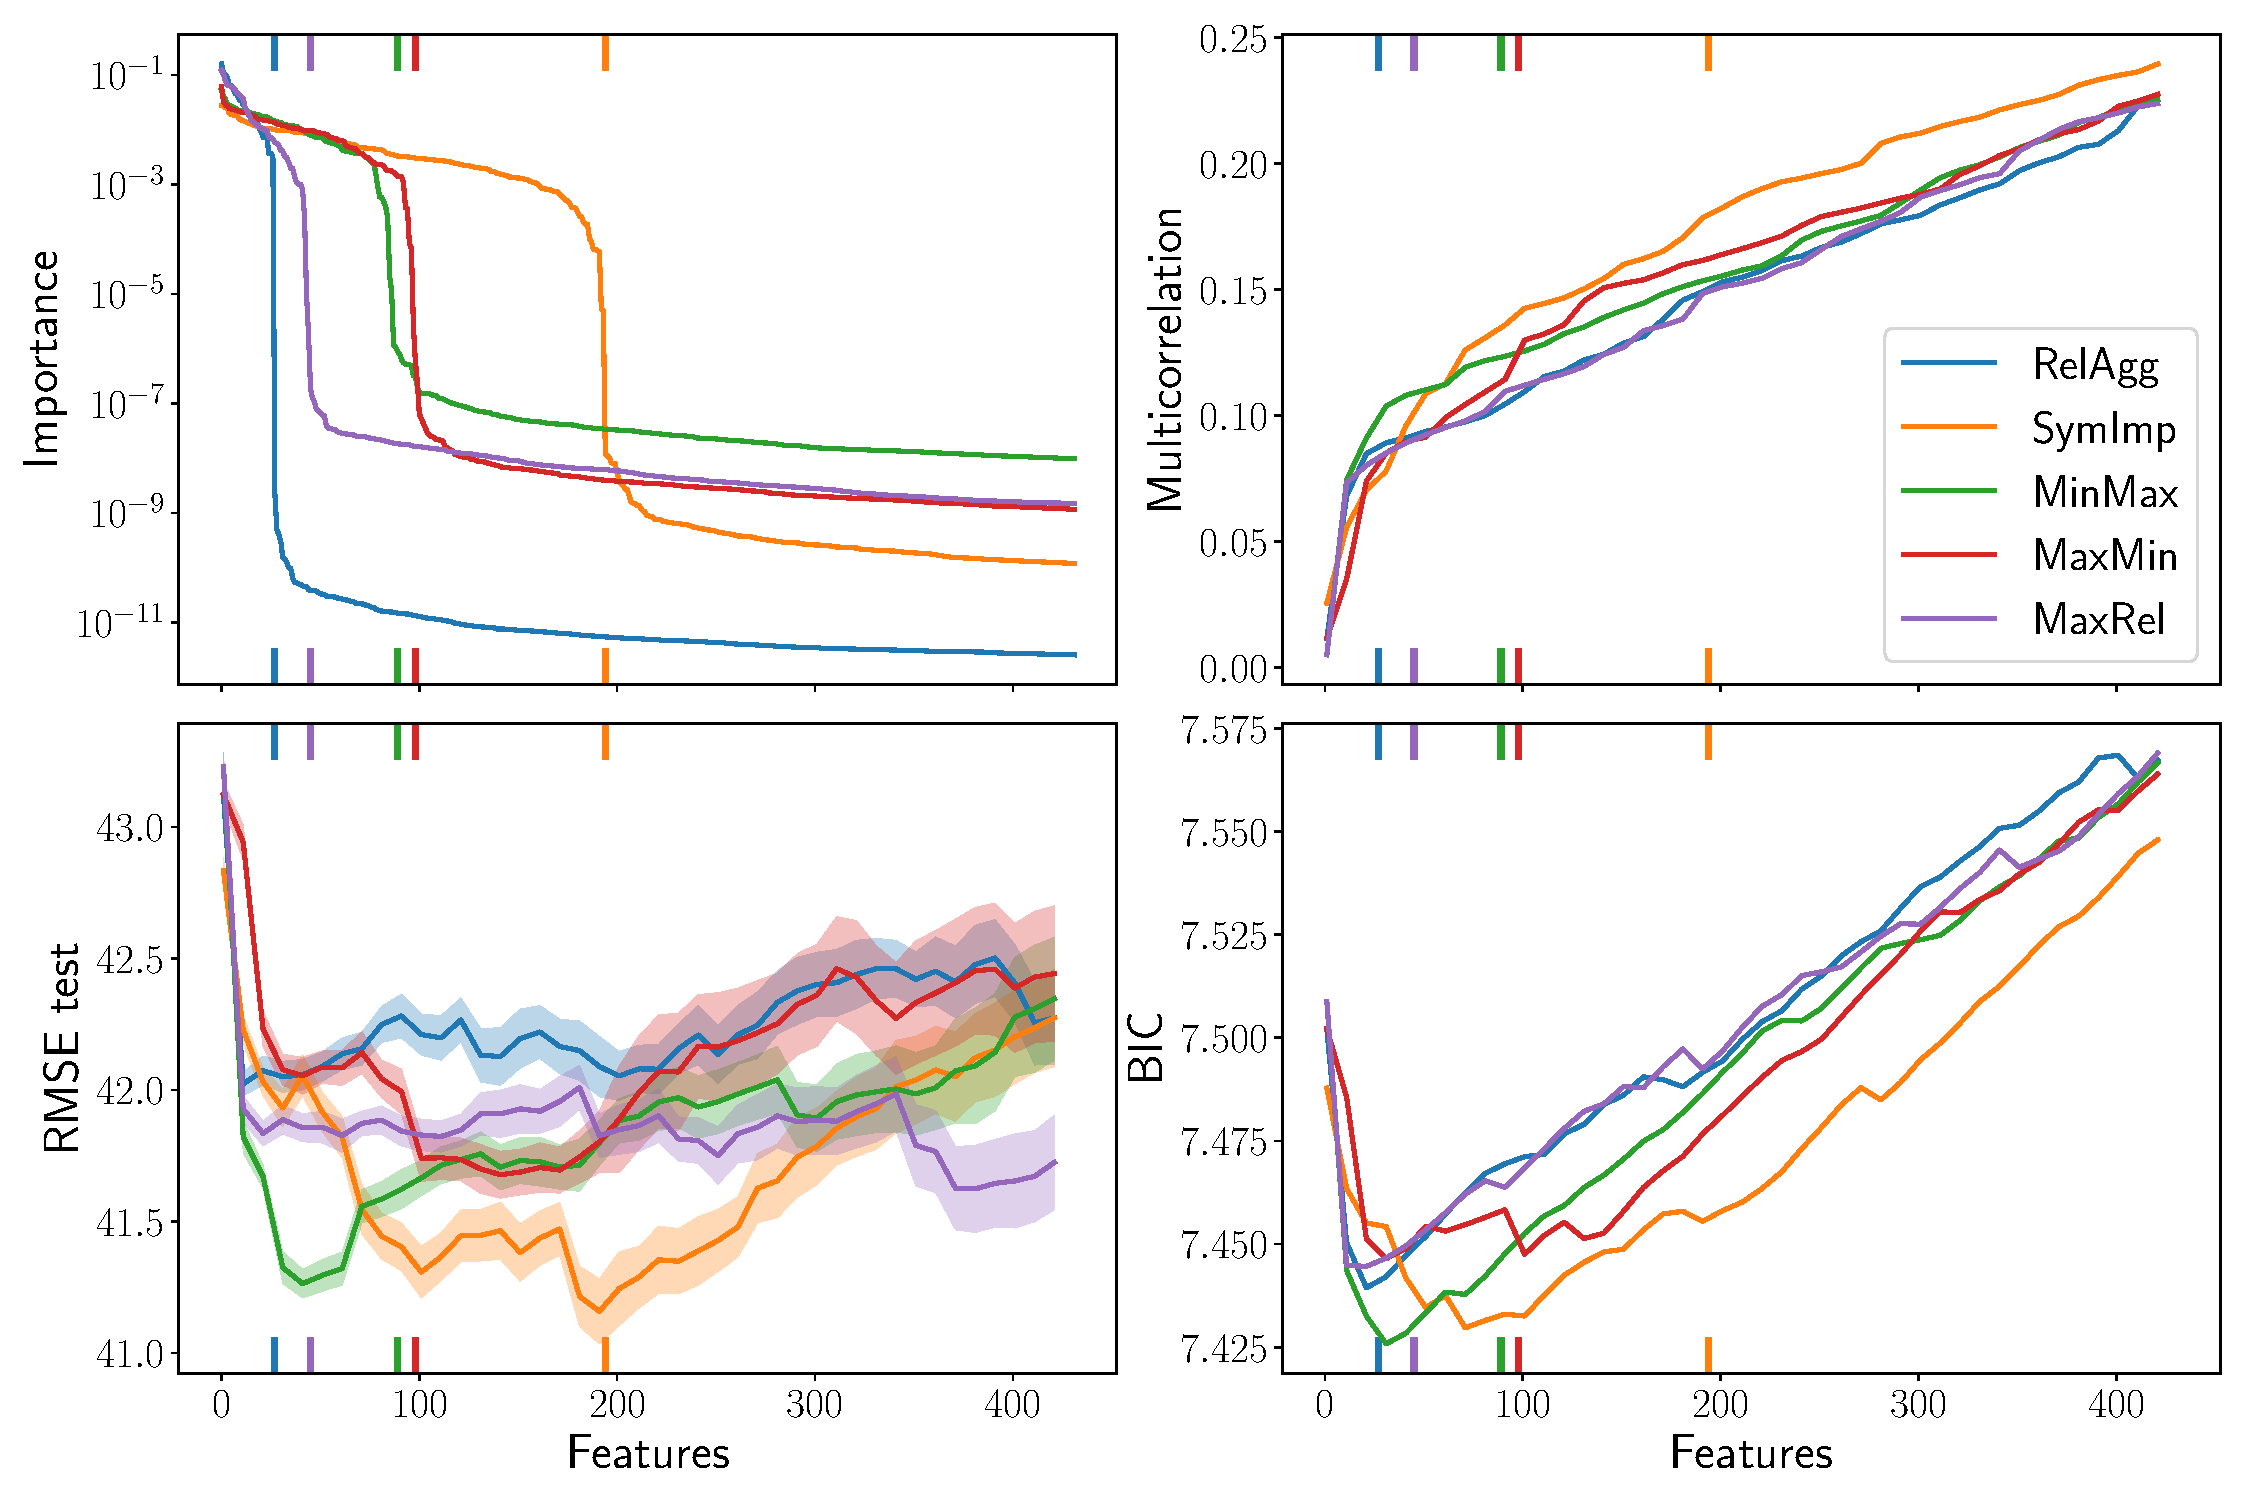
\includegraphics[width=\linewidth]{figs/ecog_3_18_metrics.pdf}
	\end{figure}
\end{frame}

%--------------------------------------------------------------------------------
\begin{frame}{Stability of selected feature subsets}
\begin{block}{Experiment design}
	\begin{itemize}
	\item generate bootstrap data
	\vspace{-0.1cm}
	\[
		(\bX, \bY) \rightarrow \bigl\{(\bX_1, \bY_1), \dots, (\bX_s, \bY_s)\bigr\};
	\]
	\item solve feature selection problem 
	\vspace{-0.1cm}
	\[
		 \bigl\{(\bX_1, \bY_1), \dots, (\bX_s, \bY_s)\bigr\}  \rightarrow \{\bz_1, \dots, \bz_s\};
	\]
	\item calculate statistics
	\vspace{-0.1cm}
	\end{itemize}
	\[
		\{\bz_1, \dots, \bz_s\} \rightarrow \{ \text{RMSE}, \|\ba\|_0, \text{Spearman }\rho, \ell_2 \text{ dist}\}.
	\]
\end{block}
\renewcommand{\arraystretch}{1.2}
\begin{table}[]
	\centering
	\begin{tabular}{l|ccccc}
		\hline
		& RMSE  & $\|\ba\|_0$ & Spearman $\rho$ & $\ell_2$ dist \\ \hline
		RelAgg & 41.9 $\pm$ 0.1 & 27.0 $\pm$ 2.4 & 0.941 $\pm$ 0.005 & 0.14 $\pm$ 0.02   \\
		SymImp & 41.1 $\pm$ 0.1 & 198.6 $\pm$ 3.8 & 0.942 $\pm$ 0.008 & 0.03 $\pm$ 0.00   \\
		MinMax & 41.4 $\pm$ 0.2 & 92.4 $\pm$ 8.2 & 0.933 $\pm$ 0.007 & 0.10 $\pm$ 0.01   \\
		MaxMin & 41.7 $\pm$ 0.1 & 97.0 $\pm$ 4.4 & 0.950 $\pm$ 0.004 & 0.07 $\pm$ 0.01   \\
		MaxRel & 41.7 $\pm$ 0.0 & 37.6 $\pm$ 1.6 & 0.893 $\pm$ 0.012 & 0.17 $\pm$ 0.02  \\ \hline
	\end{tabular}
\end{table}
\end{frame}
%--------------------------------------------------------------------------------
\begin{frame}{Conclusion}
	\begin{itemize}
		\item BCI signal decoding problem is investigated.
		\item Feature selection algorithms for multivariate spatio-temporal data are proposed.
		\item Suggested algorithms are explored and compared.
	\end{itemize}
	\begin{block}{Publications}
		\begin{itemize}
			\item Isachenko~R. et al. Feature Generation for Physical Activity Classification. \emph{Artificial Intellegence and Decision Making}, submitted.
			\item Isachenko~R., Strijov~V. Quadratic programming optimization for Newton method. \emph{Lobachevskii Journal of Mathematics}, accepted.
			\item Isachenko~R., Vladimirova~M., Strijov~V. Dimensionality reduction for time series decoding and forecasting problems. Ready for submission.
		\end{itemize}
	\end{block}
\end{frame}
\end{document} 
